%%%%%%%%%%%%%%%%%%%%%%%%%%%%%%%%%%%%%%%%%
% Fancyslides Presentation
% LaTeX Template
% Version 1.0 (30/6/13)
%
% This template has been downloaded from:
% http://www.LaTeXTemplates.com
%
% The Fancyslides class was created by:
% Paweł Łupkowski (pawel.lupkowski@gmail.com)
%
% License:
% CC BY-NC-SA 3.0 (http://creativecommons.org/licenses/by-nc-sa/3.0/)
%
%%%%%%%%%%%%%%%%%%%%%%%%%%%%%%%%%%%%%%%%%

%----------------------------------------------------------------------------------------
%	PACKAGES AND OTHER DOCUMENT CONFIGURATIONS
%----------------------------------------------------------------------------------------

\documentclass{fancyslides}

\usepackage[utf8]{inputenc} % Allows the usage of non-english characters
\usepackage{times} % Use the Times font
\usepackage{booktabs} % Allows the use of \toprule, \midrule and \bottomrule in tables
\graphicspath{{images/}} % Location of the slide background and figure files

% Beamer options - do not change
\usetheme{default} 
\setbeamertemplate{navigation symbols}{} % Disable the slide navigation buttons on the bottom of each slide
\setbeamercolor{structure}{fg=\yourowntexcol} % Define the color of titles and fixed text elements (e.g. bullet points)
\setbeamercolor{normal text}{fg=\yourowntexcol} % Define the color of text in the presentation

%------------------------------------------------
% COLORS
% The following colors are predefined in this class: white, black, gray, blue, green and orange

% Define your own color as follows:
%\definecolor{pink}{rgb}{156,0,151}

\newcommand{\structureopacity}{0.75} % Opacity (transparency) for the structure elements (boxes and circles)

\newcommand{\strcolor}{blue} % Set the color of structure elements (boxes and circles)
\newcommand{\yourowntexcol}{white} % Set the text color

%----------------------------------------------------------------------------------------
%	TITLE SLIDE
%----------------------------------------------------------------------------------------

\newcommand{\titlephrase}{A LONG AND COMPLICATED PRESENTATION TITLE} % Presentation title
\newcommand{\name}{John Smith} % Presenter's name
\newcommand{\affil}{UCLA} % Presenter's institution
\newcommand{\email}{john@LaTeXTemplates.com} % Presenter's email address

\begin{document}

\startingslide % This command inserts the title slide as the first slide

%----------------------------------------------------------------------------------------
%	PRESENTATION SLIDES
%----------------------------------------------------------------------------------------

\fbckg{1.jpg} % Slide background image
\begin{frame}
\pointedsl{main point} % Text in this environment is printed in a circle and will be made large and uppercase - if you need to fit more text in you can reduce the font size within the \pointedsl{} bracket as usual, e.g. \pointedsl{\large smaller main point}
\end{frame}

%------------------------------------------------

\fbckg{2.jpg} % Slide background image
\begin{frame}
\framedsl{explained clearly with more text} % Text in this environment will be made large, uppercase and will wrap multiple lines
\end{frame}

%------------------------------------------------

\fbckg{2.jpg} % Slide background image
\begin{frame}
\itemized{ % This environment simply prints a series of bullet points
\item or as a list containing multiple points
\item alternatively, you may want a few main points appearing one by one\ldots
}
\end{frame}

%------------------------------------------------

\fbckg{2.jpg} % Slide background image
\begin{frame}
\framedsl{\pitem{First point} \pitem{Second point} \fitem{Third point}} % Text in \pitem commands will be printed one after another on separate slides until all are displayed
\end{frame}

%------------------------------------------------

\fbckg{2.jpg} % Slide background image
\begin{frame}
\misc{ % Anything can be placed inside the \misc{} command
\Huge
Numbered list:
\begin{enumerate}
\centering
\item First item
\item Second item
\item Third item
\end{enumerate}
}
\end{frame}

%------------------------------------------------

\fbckg{2.jpg} % Slide background image
\begin{frame}
\misc{ % Anything can be placed inside the \misc{} command
Tables can be included with the \texttt{\textbackslash misc\{\}} command:
\begin{table}[h]
\begin{tabular}{l l l}
\toprule
\textbf{Treatments} & \textbf{Response 1} & \textbf{Response 2}\\
\midrule
Treatment 1 & 0.0003262 & 0.562 \\
Treatment 2 & 0.0015681 & 0.910 \\
Treatment 3 & 0.0009271 & 0.296 \\
\bottomrule
\end{tabular}
\end{table}
}
\end{frame}

%------------------------------------------------

\fbckg{2.jpg} % Slide background image
\begin{frame}
\misc{ % Anything can be placed inside the \misc{} command
Figures can also be included with the \texttt{\textbackslash misc\{\}} command:
\begin{figure}[h]

\includegraphics[width=0.4\linewidth]{placeholder}
\end{figure}
}
\end{frame}

%------------------------------------------------

\fbckg{1.jpg} % Slide background image
\begin{frame}
\thankyou % Inserts a thank you slide
\end{frame}

%------------------------------------------------

\fbckg{blank} % A blank background can be used instead of an image
\begin{frame}
\sources{ % An environment for giving credit for slide backgrounds, images will need to be scaled down if there are more than two
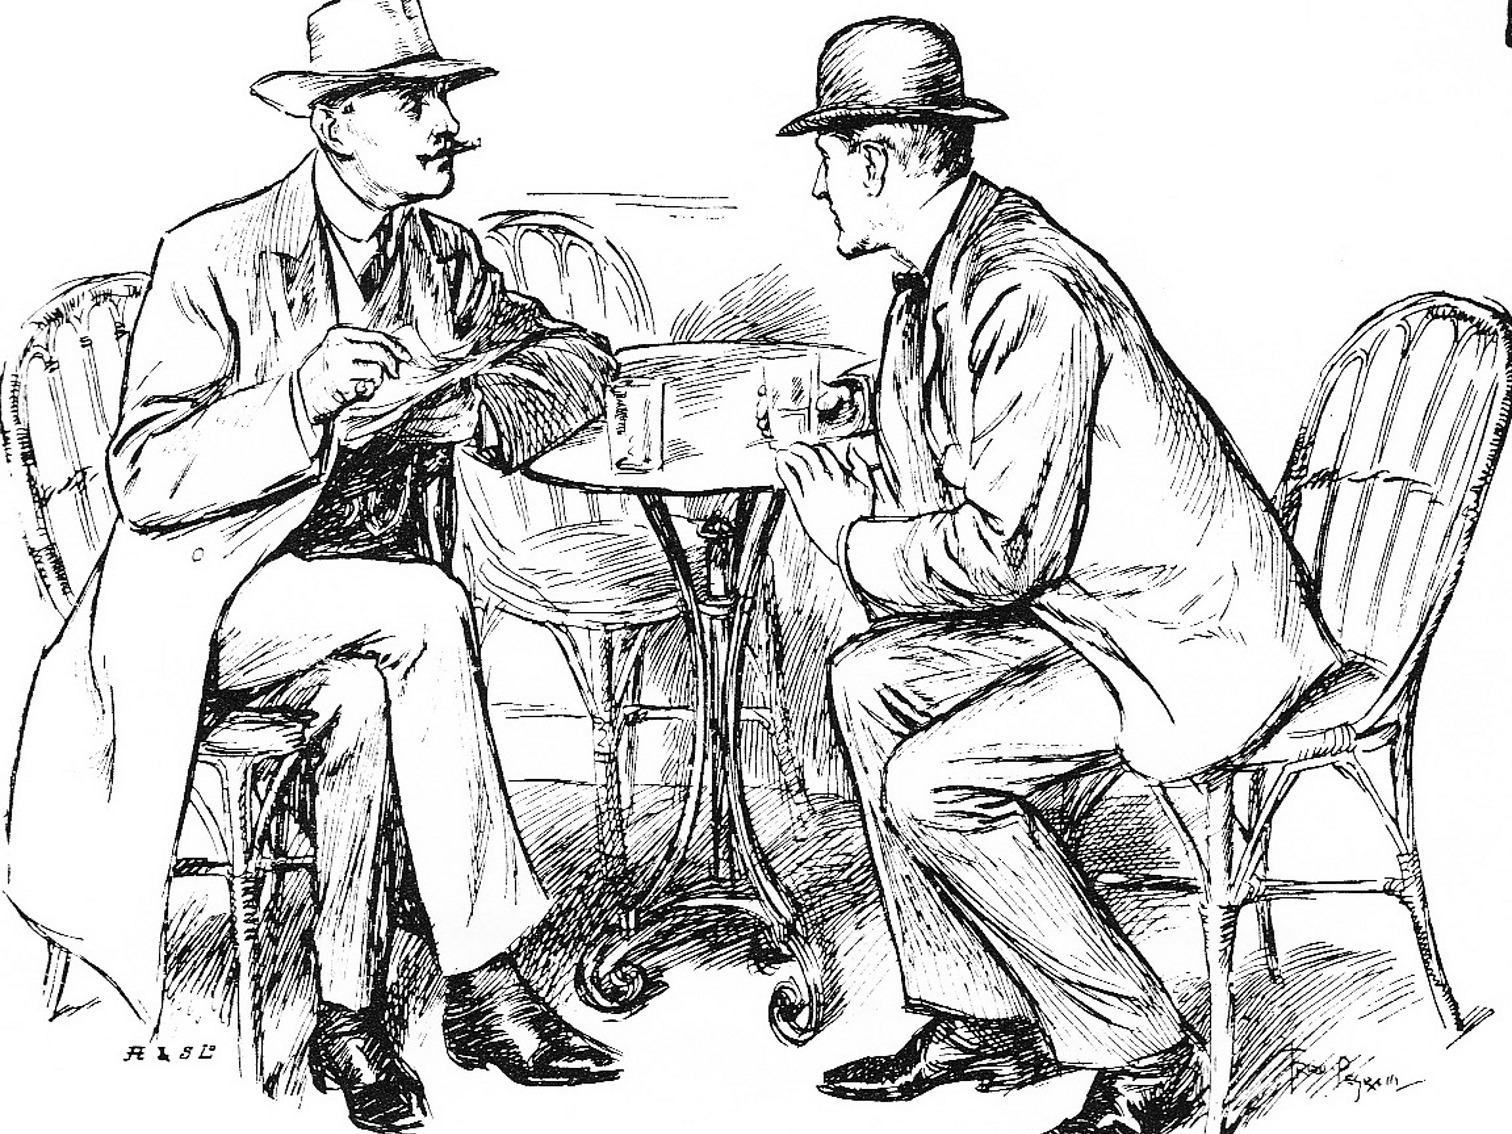
\includegraphics[scale=0.048]{1.jpg} \ flickr/lovelornpoets\\
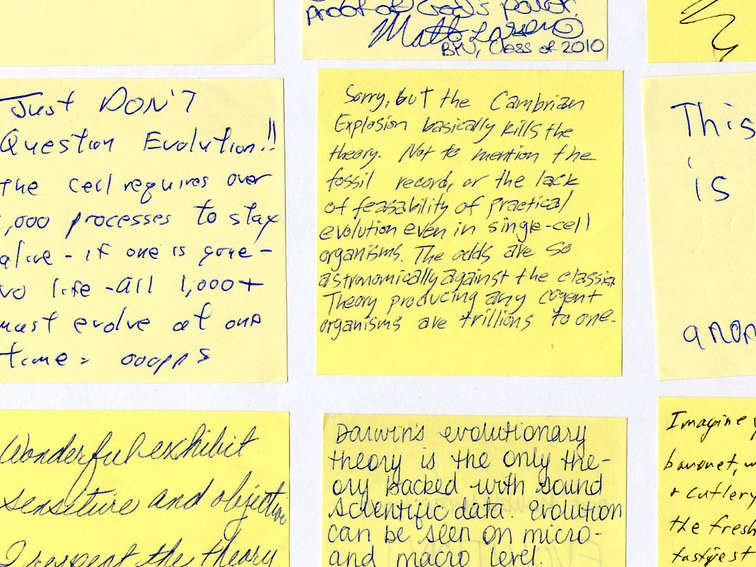
\includegraphics[scale=0.2]{2.jpg} \ flickr/apsmuseum
}
\end{frame}

%----------------------------------------------------------------------------------------

\end{document}